%!TEX root=../../Benutzerhandbuch.tex
\section{Backtestingsoftware}

Die \gls{BTS} ist nun also die Kernsoftware, mit der die Algorithmen über Daten-Files getestet werden können. Dazu sollten zuerst die allgemeinen Einstellungen getätigt werden. Diese befinden sich im Settings-Tab unter ''Orders'' und sehen so aus:

\begin{figure}[H]
\centering
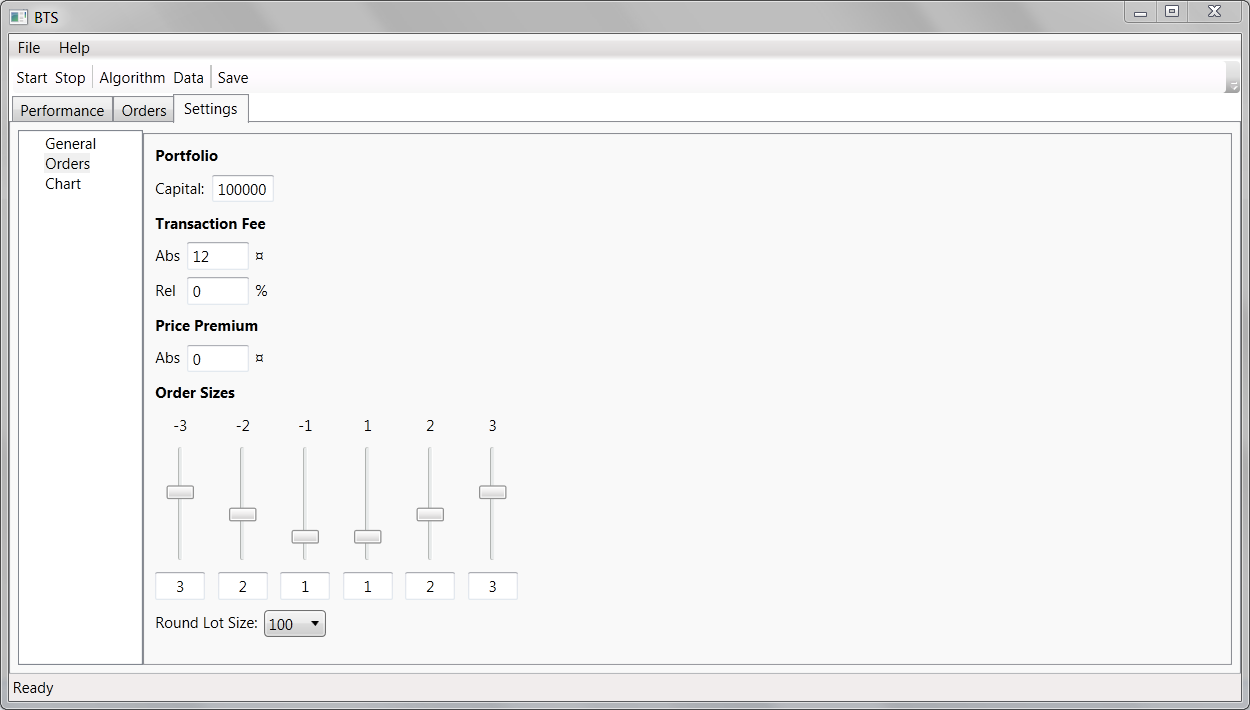
\includegraphics[width=1\textwidth]{images/btsordersettings.png}
\caption{Order-Settings der \gls{BTS}}
\end{figure}

Hier kann zuerst das gewünschte Kapital eingestellt werden, dessen Handel die \gls{BTS} simulieren soll. Danach können Transaktionsgebühren absolut oder relativ, ein Preisaufschlag für Käufe und die Order-Größen eingestellt werden. Die Order-Größen geben an, wie viele Round Lots bei einem Signal von -3 bis +3 gekauft/verkauft werden sollen. Ein Round Lot ist hierbei die kleinste über einen Online-Broker erwerbbare Menge an Aktien, die ebenfalls variieren und daher eingestellt werden kann.\\ \\

Auf der Seite darunter, der ''Chart''-Seite, können verschiedene Indikatoren aus der Combobox ausgewählt und hinzugefügt werden, die dann nach der Performancemessung in die Grafik im Orders-Tab eingezeichnet werden. Hier können außerdem für jeden Indikator die entsprechend notwendigen Parameter und Farben ausgewählt werden.

\begin{figure}[H]
\centering
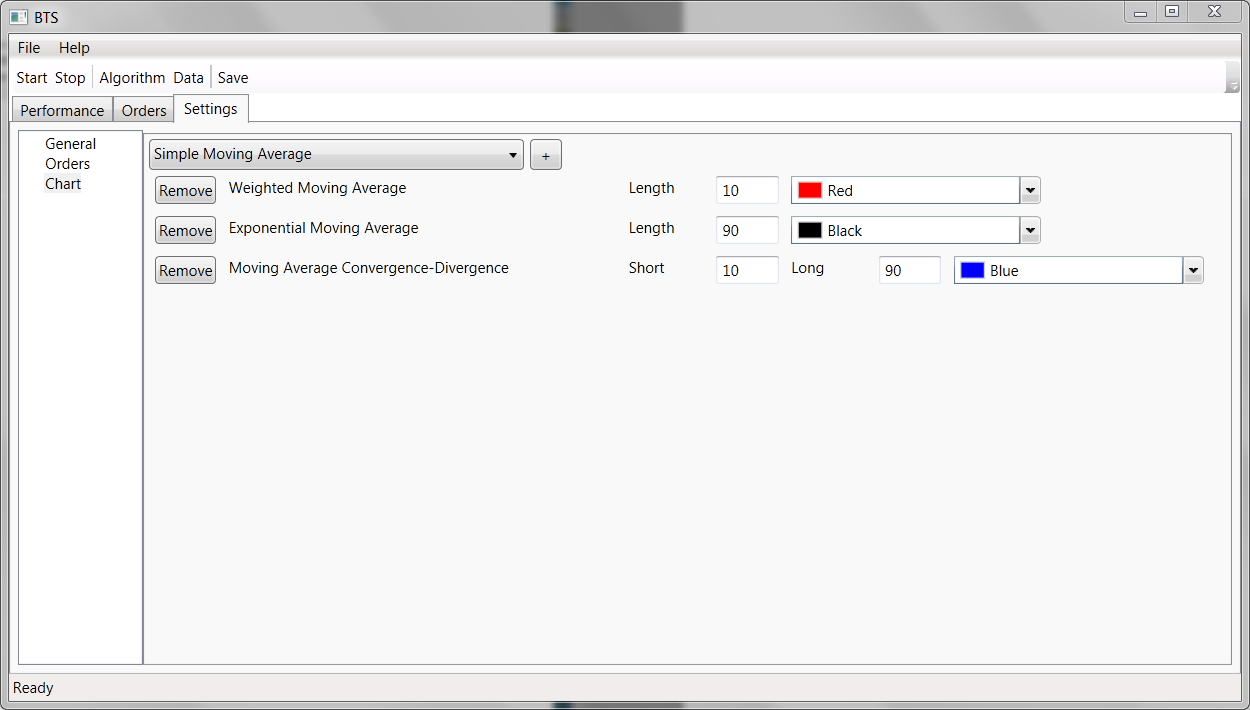
\includegraphics[width=1\textwidth]{images/btschartsettings.png}
\caption{Chart-Settings der \gls{BTS}}
\end{figure}

Weiters können nun unter der Seite ''General'' die eigentlich wichtigsten Informationen festgelegt werden. Diese sind die Pfade zur Algorithmus- und zur Daten-Datei, die in den vorherigen Punkten erläutert wurden. Diese Pfade können übrigens auch durch den ''Algorithm''- und den ''Data''-Button in der Menüleiste hinzugefügt werden. Darunter kann noch eine Zeitspanne ausgewählt werden. Der Algorithmus wird dann nur über alle Daten getestet, die im Daten-File im gewählten Zeitraum vorkommen.

\begin{figure}[H]
\centering
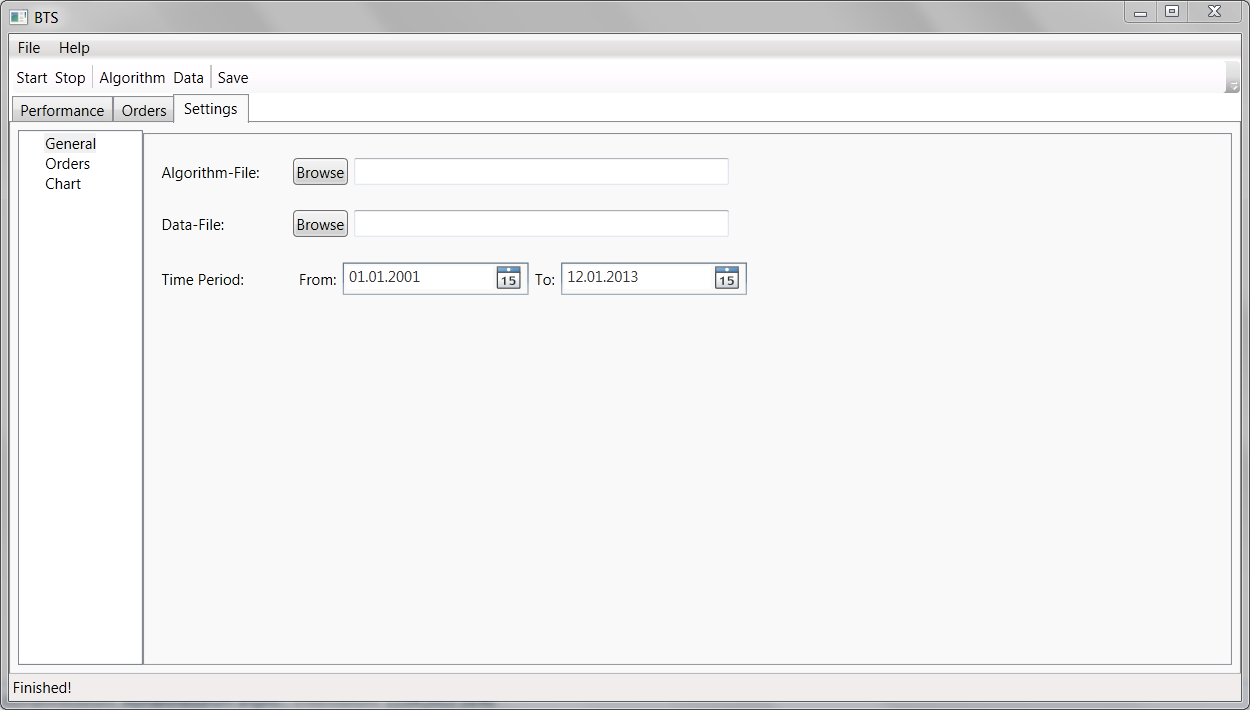
\includegraphics[width=1\textwidth]{images/btsgeneralsettings.png}
\caption{General-Settings der \gls{BTS}}
\end{figure}

Nachdem alle Einstellungen getroffen wurden, kann der Test gestartet werden.

\begin{figure}[H]
\centering
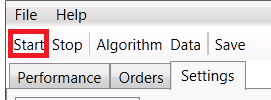
\includegraphics[width=0.6\textwidth]{images/btsstart.png}
\caption{Start-Button der \gls{BTS}}
\end{figure}

Anschließend werden auf dem Performance-Tab der \gls{BTS} die allgemeinen Performance-Daten des Algorithmus über das spezifizierte Daten-File ausgegeben. Nähere Erklärungen zu diesen Werten können durch Halten der Maus über einen der Texte als Tooltip angezeigt werden.

\begin{figure}[H]
\centering
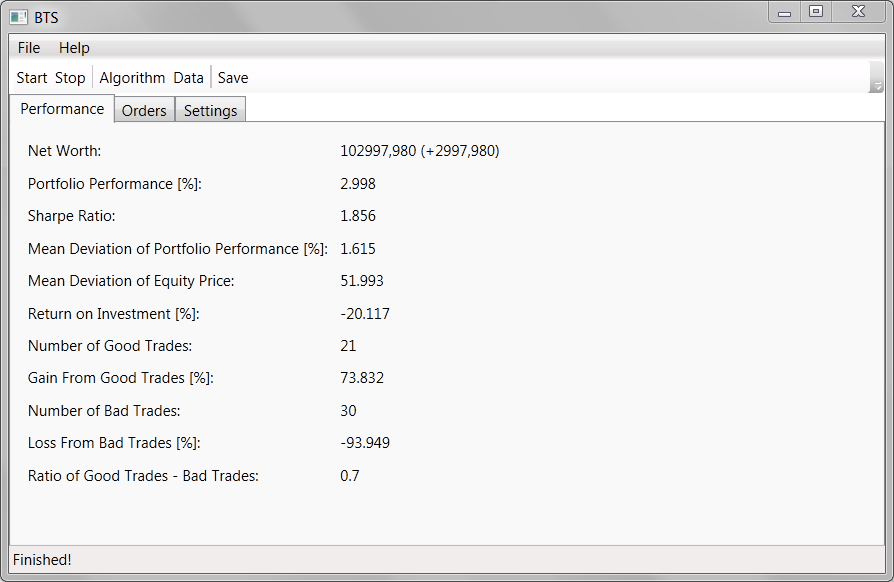
\includegraphics[width=1\textwidth]{images/btsperformance.png}
\caption{Start-Button der \gls{BTS}}
\end{figure}

Die meisten Informationen über den Verlauf des Tests können nun auf dem Orders-Tab gefunden werden. Hier wird zuerst oben ein Chart der Aktien-Preisdaten mit allen gewählten Indikatoren angezeigt. Durch Rechtsklick mit der Maus kann im Chart hinausgezoomt und mit der linken Maustaste hineingezoomt werden. Die Pfeile im Chart zeigen an, zu welchen Zeitpunkten der Algorithmus unter reellen Bedingungen über den gewählten Zeitabschnitt Signale ausgegeben hätte. Die unterschiedlichen Farben und Farbschattierungen zeigen dabei ein Kauf- (Grün) oder ein Verkauf-Signal (Rot) und dessen Stärke an.\\
In der unteren Hälte des Bildschirms wird zu jedem dieser Signale ausgegeben welchen Effekt das jeweilige Signal auf das Kapital hätte und welcher Gewinn oder Verlust dadurch zum damaligen Preis entstanden wäre. Position bzw. der Transaction Price geben dabei an, wieviele Round Lots durch dieses Signal gekauft worden wären und wieviel die Umsetzung des Signals kosten würde. Gain/Loss bezieht sich auf die prozentuelle Veränderung des Investitionskapitals der expliziten Order und Portfolio Performance auf die prozentuelle bzw. absolute Veränderung des gesamten gewählten Kapitals. All diese Werte werden auch kumulativ, also aufaddiert, angezeigt. 

\begin{figure}[H]
\centering
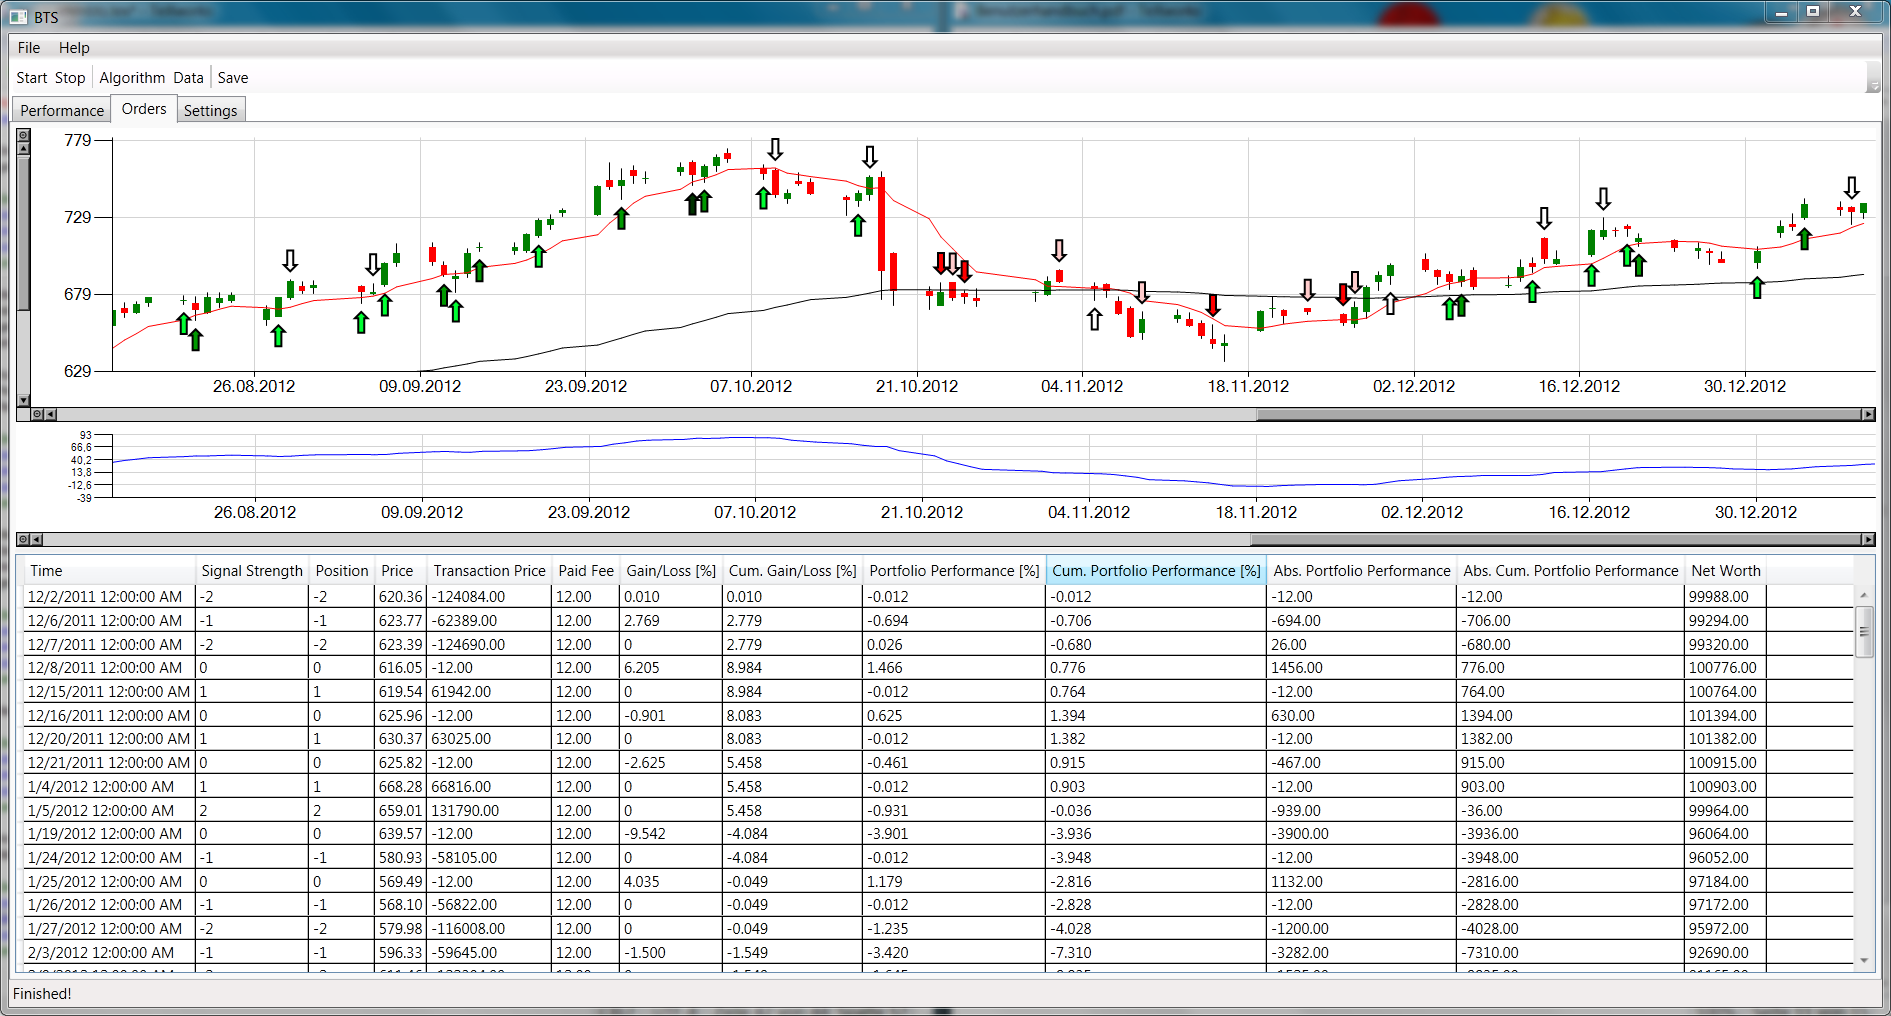
\includegraphics[width=1\textwidth]{images/btsorders.png}
\caption{Start-Button der \gls{BTS}}
\end{figure}

Zu guter Letzt können unter ''File'' -> ''Export'' die berechneten Performance-Daten lesbar als Text-File (.txt) exportiert werden. Außerdem kann der aktuelle Zustand der \gls{BTS} inklusive aller Settings und berechneter Daten außer der Charts (da sonst die Aktiendaten mitgespeichert werden müssten) gespeichert und zu einem späteren Zeitpunkt erneut geladen werden.